\documentclass[11pt,a4paper]{article}

% ---------- FONTS & ENCODING ----------
\usepackage{fontspec}
\setmainfont{TeX Gyre Pagella}
\setsansfont{TeX Gyre Heros}

% ---------- LAYOUT & PACKAGES ----------
\usepackage[a4paper,top=2.3cm,bottom=2.3cm,left=2.6cm,right=2.6cm]{geometry}
\usepackage[table]{xcolor}
\usepackage{graphicx}
\usepackage{tikz}
\usetikzlibrary{shapes.geometric}
\usepackage{titlesec}
\usepackage{tcolorbox}
\tcbuselibrary{skins,breakable}
\usepackage{booktabs}
\usepackage{array}
\usepackage{longtable}
\usepackage{enumitem}
\usepackage{fancyhdr}
\usepackage{hyperref}
\usepackage{ragged2e}
\usepackage{xstring}
\usepackage{setspace}
\usepackage{pgfgantt} % Added for the project timeline

% ---------- BRAND COLORS (Palette A: Navy & Amber) ----------
\definecolor{navy}{HTML}{1B2A6B}
\definecolor{navydark}{HTML}{10193F}
\definecolor{amber}{HTML}{F2994A}
\definecolor{ink}{HTML}{1A1A1A}
\definecolor{softgray}{HTML}{6E6E6E}
\definecolor{mutedblue}{HTML}{9AA6CE}
\definecolor{linegray}{HTML}{E7E7E7}
\definecolor{tabletint}{HTML}{F8F9FC} % Ultra-subtle structural tint

\hypersetup{colorlinks=true, linkcolor=ink, urlcolor=navy}

% ---------- SECTION STYLE (High-End Agency Design) ----------
% Large Amber Number | Navy Title, anchored by a dual-tone underline
\titleformat{\section}
  {\normalfont\bfseries\fontsize{19}{24}\selectfont\color{navydark}}
  {\textcolor{amber}{\fontsize{24}{24}\selectfont\thesection}\hspace{0.5em}\textcolor{linegray}{\rule[-2pt]{1.5pt}{18pt}}\hspace{0.2em}}
  {0em}
  {}
  [\vspace{6pt}\rlap{\textcolor{amber}{\rule{2.5cm}{1.5pt}}}\textcolor{linegray}{\rule{\linewidth}{0.5pt}}]
\titlespacing*{\section}{0pt}{2.4em}{1.2em}

% Subsection: Clean matching Amber number
\titleformat{\subsection}
  {\normalfont\bfseries\fontsize{13}{16}\selectfont\color{navy}}
  {\textcolor{amber}{\thesubsection}}
  {0.8em}
  {}
\titlespacing*{\subsection}{0pt}{2em}{1em}

% ---------- HEADER / FOOTER (single hairline, minimal) ----------
\pagestyle{fancy}
\fancyhf{}
\renewcommand{\headrulewidth}{0pt}
\renewcommand{\footrulewidth}{0pt}
\fancyhead[L]{\fontsize{7.6}{10}\selectfont\color{softgray}\textsc{Agam AI Labs}}
\fancyhead[R]{\fontsize{7.6}{10}\selectfont\color{softgray}\textsc{Allocabs App -- Review Report}}
\fancyfoot[L]{\fontsize{7.6}{10}\selectfont\color{softgray}\textsc{Confidential}}
\fancyfoot[R]{\fontsize{7.6}{10}\selectfont\color{amber}\thepage}
\renewcommand{\headrule}{{\color{linegray}\hrule height 0.6pt}}


% =====================================================
% ---------- UI/UX ELEMENTS: BRAND-ALIGNED CHIPS ----------
% =====================================================

% Base macro for crisp UI chips
\newtcbox{\uibadge}[3][navy]{on line, arc=2.5pt, colback=#2, colframe=#1, boxrule=0.5pt,
  fontupper=\bfseries\sffamily\fontsize{7.5}{7.5}\selectfont,
  colupper=#3, boxsep=0pt, left=6pt, right=6pt, top=3pt, bottom=3pt}

% Severity badges for inline lists (100% Brand Palette)
\newcommand{\severity}[1]{%
  \ifstrequal{#1}{High}{\uibadge[navydark]{navydark}{white}{High priority}}{%
  \ifstrequal{#1}{Medium}{\uibadge[amber]{amber!15}{navydark}{Medium priority}}{%
  \uibadge[mutedblue]{mutedblue!15}{navydark}{Low priority}}}%
}

% Short priority badges for table cells (100% Brand Palette)
\newcommand{\pri}[1]{%
  \ifstrequal{#1}{High}{\uibadge[navydark]{navydark}{white}{High}}{%
  \ifstrequal{#1}{Medium}{\uibadge[amber]{amber!15}{navydark}{Medium}}{%
  \uibadge[mutedblue]{mutedblue!15}{navydark}{Low}}}%
}

% Premium solid-color table headers
\newcommand{\thd}[1]{\textsc{\bfseries\color{white}\fontsize{8.6}{8.6}\selectfont #1}}


% =====================================================
% ---------- CALLOUT BLOCKS (Sharp Modern Shadows & Mini-Chips) ----------
% =====================================================

\newtcolorbox{issuebox}[2]{
  enhanced, colback=white, colframe=linegray, boxrule=0.5pt,
  borderline west={4pt}{0pt}{navy}, % Striking solid Navy left edge
  arc=2pt, outer arc=2pt, breakable, 
  top=14pt, bottom=14pt, left=16pt, right=16pt,
  before skip=18pt, after skip=18pt,
  shadow={3pt}{-3pt}{0pt}{navy!10}, % Crisp, sharp unblurred shadow for depth
  before upper={%
    % Mini-chip for the Subtitle / Category
    \tcbox[on line, boxsep=0pt, boxrule=0pt, colback=navy!8, colframe=navy!8, left=5pt, right=5pt, top=3pt, bottom=3pt, arc=2pt]{\sffamily\bfseries\fontsize{8}{10}\selectfont\color{navy}\MakeUppercase{#1}}\\[8pt]
    {\bfseries\fontsize{14}{16}\selectfont\color{navydark}#2}\\[6pt]
    {\color{linegray}\hrule height 0.5pt}\vspace{10pt}
  }
}

\newtcolorbox{recbox}[2]{
  enhanced, colback=white, colframe=linegray, boxrule=0.5pt,
  borderline west={4pt}{0pt}{amber}, % Striking solid Amber left edge
  arc=2pt, outer arc=2pt, breakable, 
  top=14pt, bottom=14pt, left=16pt, right=16pt,
  before skip=18pt, after skip=18pt,
  shadow={3pt}{-3pt}{0pt}{amber!15}, % Crisp, sharp unblurred shadow for depth
  before upper={%
    % Mini-chip for the Subtitle / Category
    \tcbox[on line, boxsep=0pt, boxrule=0pt, colback=amber!15, colframe=amber!15, left=5pt, right=5pt, top=3pt, bottom=3pt, arc=2pt]{\sffamily\bfseries\fontsize{8}{10}\selectfont\color{amber!90!black}\MakeUppercase{#1}}\\[8pt]
    {\bfseries\fontsize{14}{16}\selectfont\color{navydark}#2}\\[6pt]
    {\color{linegray}\hrule height 0.5pt}\vspace{10pt}
  }
}

% Clean tech-style bullet points (tiny squares)
\setlist[itemize]{label=\textcolor{amber}{\rule{3.5pt}{3.5pt}}, leftmargin=1.8em, itemsep=7pt, topsep=8pt}
\setlist[enumerate]{label=\textbf{\textcolor{navy}{\arabic*.}}, leftmargin=1.8em, itemsep=7pt, topsep=8pt}
\setstretch{1.18}
\arrayrulecolor{linegray}

% =====================================================
\begin{document}

% ================= COVER PAGE =================
\begin{titlepage}
\newgeometry{margin=0cm}
\begingroup
\pagecolor{navy}
\color{white}

\begin{tikzpicture}[remember picture, overlay]
  \fill[navy] (current page.north west) rectangle (current page.south east);

  \draw[amber!55, line width=0.9pt]
     ([xshift=-2cm,yshift=1.5cm]current page.south west) to[out=70,in=200]
     ([xshift=4cm,yshift=9cm]current page.south west) to[out=20,in=250]
     (current page.north east);
  \draw[mutedblue, line width=0.5pt, opacity=0.35]
     ([xshift=1cm,yshift=0cm]current page.south west) to[out=75,in=205]
     ([xshift=6cm,yshift=10.5cm]current page.south west) to[out=25,in=250]
     ([xshift=-1cm]current page.north east);

  \node[anchor=north west, fill=white, rounded corners=3pt, inner sep=9pt]
     at ([xshift=2.6cm,yshift=-2.6cm]current page.north west)
     {
\includegraphics[width=2.3cm]{../../Images/agamailabs.png}};

  \draw[amber, line width=1.6pt]
     ([xshift=2.6cm,yshift=-11.6cm]current page.north west) --
     ([xshift=2.6cm,yshift=-17.9cm]current page.north west);

  \node[anchor=north west, text=amber] at ([xshift=3.15cm,yshift=-11.9cm]current page.north west)
     {\fontsize{10.5}{13}\selectfont\textsc{Confidential Review}};

  \node[anchor=north west, text=white, align=left, text width=13.8cm]
     at ([xshift=3.15cm,yshift=-13.1cm]current page.north west)
     {\fontsize{33}{39}\selectfont\bfseries Allocabs Mobile App\\ Review \& Enhancement Report};

  \node[anchor=north west, text=mutedblue, align=left, text width=11.5cm]
     at ([xshift=3.15cm,yshift=-17.3cm]current page.north west)
     {\fontsize{11.5}{16}\selectfont Issues, UX corrections, feature roadmap and timeline.};

  \node[anchor=south west, text=mutedblue, align=left, text width=15.8cm]
     at ([xshift=2.6cm,yshift=2.9cm]current page.south west)
     {\fontsize{9}{14}\selectfont\textsc{Prepared for} \ Allocabs \quad\textbullet\quad \textsc{Prepared by} \ Naveen, Agam AI Labs \quad\textbullet\quad July 10, 2026};

  \node[anchor=south west, text=mutedblue] at ([xshift=2.6cm,yshift=1.5cm]current page.south west)
     {\fontsize{8}{10}\selectfont\textsc{Ref. AGAL-2026-ALLOCABS-001.01.tex \ -- \ Client Draft}};

\end{tikzpicture}

\endgroup
\nopagecolor
\restoregeometry
\end{titlepage}

% ================= TABLE OF CONTENTS =================
\thispagestyle{empty}
\begin{center}

\includegraphics[width=2.6cm]{../../Images/agamailabs.png}
\end{center}
\vspace{0.6em}
\tableofcontents
\newpage

% ================= EXECUTIVE SUMMARY =================
\section{Executive Summary}
This report details the technical and functional audit of the Allocabs mobile platform, conducted by Agam AI Labs to identify critical friction points and growth opportunities. Our assessment uncovered \textbf{44 actionable opportunities} ranging from immediate usability and stability fixes to strategic feature expansions - all designed to strengthen platform reliability and elevate the user experience. By addressing these foundational issues alongside the implementation of our proposed automation roadmap - including AI-driven voice dispatch, automated KYC verification, and intelligent support routing - Allocabs will be positioned to significantly reduce manual operational overhead and scale efficiently. The recommendations presented here are structured into a phased, milestone-based delivery plan, enabling your team to prioritize high-impact stability improvements while concurrently advancing long-term feature innovation and expansion.

% ----- TIKZ METRIC CARDS -----
\vspace{1.5em}
\begin{center}
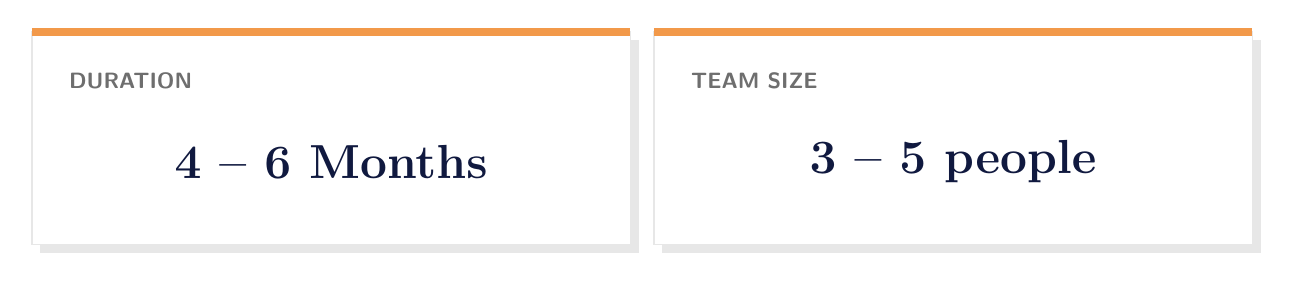
\begin{tikzpicture}
\def\cardw{7.6cm}
\def\cardh{2.7cm}
\foreach [count=\i] \cardtitle/\cardval in {Duration/{4 -- 6 Months},Team Size/{3 -- 5 people}}{
  % Crisp Drop Shadow
  \fill[linegray] ({(\i-1)*7.9cm + 3pt},-3pt) rectangle ++(\cardw,-\cardh);
  % Main White Card Frame
  \draw[linegray, line width=0.5pt, fill=white]
        ({(\i-1)*7.9cm},0) rectangle ++(\cardw,-\cardh);
  % Bold Top Accent Rule
  \draw[amber, line width=3pt]
        ({(\i-1)*7.9cm},0) -- ++(\cardw,0);
  % Subtitle / Label
  \node[anchor=north west, font=\fontsize{8.5}{10}\selectfont\sffamily\bfseries\color{softgray}]
        at ({(\i-1)*7.9cm + 0.35cm},-0.4) {\MakeUppercase{\cardtitle}};
  % Main Value
  \node[anchor=center, font=\fontsize{19}{22}\selectfont\bfseries\color{navydark}]
        at ({(\i-1)*7.9cm + \cardw/2},-1.65) {\cardval};
}
\end{tikzpicture}
\end{center}
\vspace{1.5em}

\renewcommand{\arraystretch}{1.8}
\begin{center}
{\rowcolors{2}{white}{tabletint}
\begin{tabular}{@{}p{3.2cm}p{11.3cm}@{}}
\rowcolor{navy}
\thd{Report Field} & \thd{Detailed Information} \\
\arrayrulecolor{linegray}\midrule[0.5pt]
\textbf{Scope} & UX redesign, bug fixes, new feature development, and strategic integrations for the Allocabs mobile app \\
\midrule[0.5pt]
\textbf{Engagement} & Fixed-scope project, milestone-based delivery \\
\arrayrulecolor{navy}\bottomrule[1.5pt]
\end{tabular}}
\end{center}

% ================= CURRENT STATE / ISSUES =================
\section{Current State \& Issues Identified}
All action items raised during the walkthrough are explained below, grouped strictly into three main categories: \textbf{Existing Issues}, \textbf{Enhancement and Expansion}, and \textbf{Agam AI Labs Suggestions}.

\subsection{Existing Issues}
\begin{issuebox}{Audit Findings}{Existing Issues Identified}
\begin{itemize}
  \item \textbf{On-Duty Toggle:} Small tap target with a delayed response, so a repeat tap can flip it twice. \severity{Medium}
  \item \textbf{Notification Sound:} Uses media volume instead of ringtone volume. \severity{High}
  \item \textbf{Android Notifications:} Not reliably delivered on most Android devices. \severity{High}
  \item \textbf{Location Pin Bug:} Pin shifts to a new spot if the map is moved after placement. \severity{Medium}
  \item \textbf{Phone Number Validation:} Phone number field accepts numbers starting with 0. \severity{Low}
  \item \textbf{Address Display:} Source and destination text changes after selecting a location from the map instead of preserving the entered address. \severity{Medium}
  \item \textbf{Repeat Driver Offers:} A driver who rejects or times out (20s, no action) can be shown the same request again instead of a different nearby driver. \severity{High}
  \item \textbf{Password Placeholder:} Create Password screen has no placeholder (e.g. "New Allo Password"). \severity{Low}
\end{itemize}
\end{issuebox}

\subsection{Enhancement and Expansion}
\begin{issuebox}{Platform Roadmap}{Enhancement and Expansion Needs}
\begin{itemize}
  \item \textbf{Booking Pop-up:} Drivers need to open the app to review booking details, leaving less time within the 20-second acceptance window. \severity{High}
  \item \textbf{Active Ride Visibility:} Ongoing booking and its status stay hidden in a background tab when the app is minimised. \severity{Medium}
  \item \textbf{Early Booking UX:} No clear interface for a dynamic acceptance window based on the trip's travel duration. \severity{Medium}
  \item \textbf{Incentive Animation:} Incentives screen has no visual progress motivation for drivers. \severity{Low}
  \item \textbf{Dispatch Delay:} Driver receives the booking request roughly 9 seconds after the user books. \severity{High}
  \item \textbf{Wallet History:} Each wallet history entry lacks clear transaction information. \severity{Medium}
  \item \textbf{One-to-One Matching:} Only one driver is offered per request; a rejection restarts the search instead of offering several drivers at once. \severity{High}
  \item \textbf{Rider Cool-down:} No auto-block for a rider whose requests are repeatedly rejected or ignored by drivers. \severity{Medium}
  \item \textbf{Cool-down Edge Case:} No fair-handling path for genuine issues (lost or broken phone) that could unfairly trigger the same block. \severity{Medium}
  \item \textbf{Peak Pricing:} No auto peak-hour but having area-based dynamic pricing alone. \severity{Medium}
  \item \textbf{Coupon Visibility:} Discount is not shown to the rider, not itemised for the driver, and cannot be scoped by vehicle, date, or usage count. \severity{Medium}
  \item \textbf{Multiple Drop-offs:} No support for multiple stops or a waiting-charge calculation. \severity{Medium}
  \item \textbf{Long-Distance Pooling \& Returns:} No option for passengers to pool long-distance rides, nor a mechanism for drivers to accept bookings specifically along their return route back to base. \severity{Medium}
  \item \textbf{Live Vehicle Rendering:} Map markers for nearby vehicles are not optimised for vehicle count or search radius. \severity{Low}
  \item \textbf{Refer \& Earn:} Link-only; no referral-code mechanism. \severity{Low}
  \item \textbf{Manual Booking:} No proper way for call-based booking path for users without the app. \severity{Medium}
  \item \textbf{KYC Management:} Profile picture and KYC documents are stored separately, with no yearly renewal or expiry alerts. \severity{High}
  \item \textbf{Multi-Device Login:} Same account can log in on more than one device; no auto-offline when GPS or network drops. \severity{Medium}
  \item \textbf{SOS Sharing:} Live tracking is visible on-screen but not shared as a link with emergency contacts. \severity{Medium}
  \item \textbf{Destination Change:} If a customer requests a different drop-off location after their phone is switched off, the driver cannot update the destination or end the ride unless they reach the original drop location. \severity{Medium}
  \item \textbf{Card Tokenisation:} Stored card details are not tokenised. \severity{Medium}
  \item \textbf{Earnings Detail:} Ride history does not display earnings for individual trips, despite earnings being available in a separate graph. \severity{Low}
  \item \textbf{Screen Wake State:} The device screen turns off while the driver app is active, interrupting continuous use. \severity{Medium}
  \item \textbf{Profile Editing Rules:} Email cannot be made optional; driver name edits go live without approval. \severity{Low}
  \item \textbf{Review Management:} Admin panel for ride reviews lacks detail and is not easy to navigate. \severity{Low}
  \item \textbf{ID Perks:} No perks or benefits tied to a passenger adding an ID. \severity{Low}
  \item \textbf{Gamification:} No driver level system (silver/gold/platinum) based on activity. \severity{Low}
  \item \textbf{Book for Someone:} No option to book a ride on behalf of another person. \severity{Low}
  \item \textbf{Wallet Withdrawal:} No constraints or automation for instant wallet withdrawals. \severity{Medium}
  \item \textbf{Post-Ride Payment:} No option to change payment method after a ride ends. \severity{Low}
  \item \textbf{BI Dashboard:} Missing advanced Business Intelligence reporting with export capabilities. \severity{Medium}
  \item \textbf{Vehicle Priority:} Vehicle list has no priority ordering (e.g. EV, bike, SUV). \severity{Low}
\end{itemize}
\end{issuebox}

\subsection{Agam AI Labs Suggestions}
\begin{issuebox}{Strategic Recommendations}{Agam AI Labs Suggestions}
\begin{itemize}
  \item \textbf{Data Privacy:} Compliance of current storage practices with data-privacy law has not been formally verified. \severity{High}
  \item \textbf{AI Automation:} Many operational workflows are handled manually today, increasing overhead as volume scales. \severity{Medium}
  \item \textbf{Beta Program:} No structured staging or beta testing group exists for rolling out new features safely before a full public launch. \severity{Medium}
  \item \textbf{Call \& Messaging:} The platform lacks phone number masking, in-app chat, and in-app calling, requiring users to share personal contact details. \severity{Medium}
\end{itemize}
\end{issuebox}

% ================= PROPOSED SOLUTION =================
\section{Proposed Solution}
Each fix below is mapped directly to the three categories defined above for easy cross-reference.

\subsection{Existing Issues Resolutions}
\begin{recbox}{Action Plan}{Fixes for Existing Issues}
\begin{itemize}
  \item \textbf{On-Duty Toggle:} Larger tap target with immediate visual feedback, debounced in the frontend to prevent double-firing.
  \item \textbf{Notification Sound:} Route through ringtone volume; verify with device testing.
  \item \textbf{Android Notifications:} Audit native vs. custom notification handling and standardise on one reliable delivery path.
  \item \textbf{Location Pin Bug:} Lock the pin independently of subsequent map movement.
  \item \textbf{Phone Number Validation:} Prevent phone numbers that start with 0.
  \item \textbf{Address Display:} Preserve the entered source and destination text after map selection.
  \item \textbf{Repeat Driver Offers:} Tune the re-offer logic to rotate to a different nearby driver on rejection/timeout.
  \item \textbf{Password Placeholder:} Add a placeholder such as "New Allo Password" to the password field.
\end{itemize}
\end{recbox}

\subsection{Enhancement and Expansion Resolutions}
\begin{recbox}{Action Plan}{Features \& Upgrades Roadmap}
\begin{itemize}
  \item \textbf{Booking Pop-up:} Rich, actionable pop-up (fare, pickup, distance) that drivers can accept from the lock/notification screen without opening the app.
  \item \textbf{Active Ride Visibility:} Persistent banner/notification whenever the app is backgrounded; when the app is reopened, the active booking screen is shown immediately.
  \item \textbf{Early Booking UX:} Dynamic booking window tied to the ride's estimated travel duration.
  \item \textbf{Incentive Animation:} Lightweight progress animation on the incentives screen.
  \item \textbf{Dispatch Delay:} Profile the booking-to-dispatch pipeline and remove the 9 second lag.
  \item \textbf{Wallet History:} Itemise every transaction with clear detail.
  \item \textbf{One-to-One Matching:} Move to a one-to-many dispatch algorithm with concurrency-safe, race-condition-free driver selection.
  \item \textbf{Rider Cool-down:} Introduce a 6--8 hour cool-down after repeated rejections/no-response.
  \item \textbf{Cool-down Edge Case:} Add an appeal path for genuine issues (lost/broken phone) before a block applies.
  \item \textbf{Peak Pricing:} Design and implement peak-hour and area-based pricing.
  \item \textbf{Coupon Visibility:} Rebuild the coupon engine with rider-facing discount breakdowns, driver commission detail, and scoping configurations.
  \item \textbf{Multiple Drop-offs:} Add multiple stops with a defined waiting-charge algorithm.
  \item \textbf{Long-Distance Pooling \& Returns:} Implement a specialized matching algorithm for long-distance pooled rides and enable a 'return trip' mode for drivers to pick up passengers along their route home.
  \item \textbf{Live Vehicle Rendering:} Cap markers based on vehicle count and search radius.
  \item \textbf{Refer \& Earn:} Add a functional referral-code system alongside the existing link.
  \item \textbf{Manual Booking:} Enhance existing call-based booking flow handled through support staff.
  \item \textbf{KYC Management:} Unify profile and KYC documents with yearly renewal, expiry alerts, and a booking lock until renewed.
  \item \textbf{Multi-Device Login:} Restrict login to one active device; auto-offline on GPS/network loss.
  \item \textbf{SOS Sharing:} Share a live tracking link with designated emergency contacts.
  \item \textbf{Destination Change:} Ensure rides can be completed when a customer changes the drop-off location after their phone is switched off.
  \item \textbf{Card Tokenisation:} Tokenise all stored card details.
  \item \textbf{Earnings Detail:} Display earnings details for each trip within the ride history.
  \item \textbf{Screen Wake State:} Keep the device screen awake while the driver app is active.
  \item \textbf{Profile Editing Rules:} Make email optional; require admin approval for driver name changes.
  \item \textbf{Review Management:} Extend the admin panel with a clearer, more detailed review view.
  \item \textbf{ID Perks:} Define perks/benefits for passengers who add an ID.
  \item \textbf{Gamification:} Add driver activity tiers (silver/gold/platinum). \textit{Optional, per Allocabs.}
  \item \textbf{Book for Someone:} Add a book-on-behalf-of flow.
  \item \textbf{Wallet Withdrawal:} Add automated, instant withdrawals within defined limits.
  \item \textbf{Post-Ride Payment:} Allow payment-method change after a ride ends.
  \item \textbf{BI Dashboard:} Build a BI dashboard with viewing and export capability.
  \item \textbf{Vehicle Priority:} Add configurable priority ordering to the vehicle list.
\end{itemize}
\end{recbox}

\subsection{Agam AI Labs Strategic Implementation}
\begin{recbox}{Action Plan}{Strategic Implementations}
\begin{itemize}
  \item \textbf{Data Privacy:} Conduct a formal data-privacy compliance review of storage, transmission, and access practices.
  \item \textbf{AI Automation:} Integrate targeted AI agents (Voice, Vision, Support) to reduce manual work and scale operations (detailed in Section 4).
  \item \textbf{Beta Program:} Establish a structured beta-testing group of trusted drivers and frequent riders to validate new features in production before general release.
  \item \textbf{Call \& Messaging:} Implement in-app chat, and in-app calling to protect user privacy and enable secure communication.
\end{itemize}
\end{recbox}

% ================= AI AUTOMATION =================
\section{AI Automation \& Scaling Strategy}
Rather than automation for its own sake, the following use cases target specific, recurring manual workloads observed during the review - each chosen because it is technically achievable today and produces a measurable reduction in staff hours.

\subsection{Automated Booking via Phone (No App Required)}
\begin{recbox}{AI Voice}{Voice AI for call-based bookings}
Today, manual bookings rely on a human agent to answer, note details, and enter them into the dispatch system. A voice AI agent, integrated over SIP, can answer these calls directly, capture pickup/drop-off details through natural conversation, and push the booking into dispatch in real time. This removes the need for a dedicated phone-booking agent for routine requests and eliminates hold-time entirely, since the agent can take multiple calls simultaneously.
\end{recbox}

\subsection{KYC Document Verification}
\begin{recbox}{Vision AI}{Automated document extraction and validation}
KYC review currently requires a staff member to manually inspect each uploaded ID, license, or insurance document, cross-check expiry dates, and update records. An OCR/vision-based pipeline can extract the relevant fields automatically, flag mismatches or expired documents, and only route genuinely ambiguous cases to a human reviewer. This turns a multi-minute manual check into a near-instant automated pass, with staff only handling exceptions.
\end{recbox}

\subsection{Support Ticket Resolution}
\begin{recbox}{AI Support}{Automated response for common queries}
A large share of support tickets are repetitive: fare disputes, ride cancellation questions, and wallet withdrawal status checks. An AI support agent with read access to ride, wallet, and trip records can resolve these directly by pulling the relevant record and giving an accurate answer, without a support agent needing to look anything up manually. This is scoped strictly to queries with a clear factual answer in existing data; anything involving judgment or a refund decision is routed to a human.
\end{recbox}

% ================= TIMELINE =================
\section{Project Timeline (Tentative)}
The engagement is planned over \textbf{4 to 6 months}, depending on final scope confirmation and the depth of the KYC/compliance and AI automation work Allocabs chooses to include.

\begin{center}
\begin{ganttchart}[
    vgrid={draw=linegray}, hgrid={draw=linegray},
    bar/.append style={fill=navydark, rounded corners=1.5pt},
    bar height=0.55,
    bar label font=\fontsize{8}{9}\selectfont\color{ink},
    milestone/.append style={fill=amber, rounded corners=1.5pt},
    milestone label font=\fontsize{8}{9}\selectfont\bfseries\color{navydark},
    group/.append style={fill=navy, rounded corners=1.5pt},
    group label font=\fontsize{8}{9}\selectfont\bfseries\color{navydark},
    group height=0.4,
    title/.append style={fill=tabletint, draw=linegray},
    title label font=\fontsize{8}{9}\selectfont\color{navy},
    title height=1,
    y unit chart=0.75cm,
    y unit title=0.75cm
  ]{1}{24}
  \gantttitle{\textsc{Weeks}}{24} \\
  \gantttitlelist{1,...,24}{1} \\
  \ganttgroup{System Analysis \& Solution Design}{1}{4} \\
  \ganttbar{Wireframes \& audit}{1}{4} \\
  \ganttgroup{Bug Fixing}{5}{8} \\
  \ganttbar{Critical bug resolution}{5}{8} \\
  \ganttgroup{Feature \& Dispatch Development}{9}{18} \\
  \ganttbar{Dispatch \& pricing logic}{9}{13} \\
  \ganttbar{Safety, KYC \& additional features}{14}{18} \\
  \ganttgroup{QA \& Release}{19}{24} \\
  \ganttbar{Testing \& deployment}{19}{24} \\
  \ganttmilestone{Launch}{24}
\end{ganttchart}
\end{center}

% ================= RESOURCES =================
\section{Team \& Resources}
Team size will flex within the ranges below depending on the phase and final scope confirmed with Allocabs.

\vspace{0.8em}
\renewcommand{\arraystretch}{1.8}
\begin{center}
{\rowcolors{2}{white}{tabletint}
\begin{tabular}{@{}p{6.5cm}p{3cm}p{3cm}@{}}
\rowcolor{navy}
\thd{Role} & \thd{Minimum} & \thd{Maximum} \\
\arrayrulecolor{linegray}\midrule[0.5pt]
Project Manager & 1 & 1 \\
\midrule[0.5pt]
Mobile Developer (Android/iOS) & 1 & 2 \\
\midrule[0.5pt]
Backend Developer & 1 & 1 \\
\midrule[0.5pt]
QA Engineer & 0 & 1 \\
\arrayrulecolor{navy}\bottomrule[1.5pt]
\end{tabular}}
\end{center}

% ================= REQUIREMENTS FROM ALLOCABS =================
\section{Requirements from Allocabs}
To finalise scope, effort estimation, and infrastructure planning, we require the following information from the Allocabs team before kick-off.

\subsection{Tech Stack}
\begin{issuebox}{Input Needed}{Tech Stack Information}
\begin{itemize}
  \item Third-party services already integrated (payment gateway, SMS/OTP provider, maps/geolocation provider, push notification service)
  \item Tech stack used
\end{itemize}
\end{issuebox}

\subsection{Hosting \& Infrastructure Details}
\begin{issuebox}{Input Needed}{Environment \& Infrastructure}
\begin{itemize}
  \item Current hosting provider (AWS, GCP, Azure, or on-premise)
  \item Server architecture (monolith vs. microservices) and current environment setup (dev/staging/production)
  \item Existing monitoring, logging, and alerting tools in place
  \item Current data storage location and any regional/compliance constraints (data residency requirements)
\end{itemize}
\end{issuebox}

\vfill
\noindent{\color{linegray}\rule{\linewidth}{0.6pt}}\\[6pt]
\fontsize{8.3}{10}\selectfont\textcolor{softgray}{Agam AI Labs \ -- \ Confidential. Prepared exclusively for Allocabs.}

\end{document}